% A toy birth-death tree run to time T, from the toy manuscript tree in
% Paper01_AgeBDPVarEnv/BDP_Presentation.tex: one ancestor, one individual that dies before T,
% and three that survive to T (blue, red and green).
% Compile with: lualatex "\def\stage{k}% A toy birth-death tree run to time T, from the toy manuscript tree in
% Paper01_AgeBDPVarEnv/BDP_Presentation.tex: one ancestor, one individual that dies before T,
% and three that survive to T (blue, red and green).
% Compile with: lualatex "\def\stage{k}% A toy birth-death tree run to time T, from the toy manuscript tree in
% Paper01_AgeBDPVarEnv/BDP_Presentation.tex: one ancestor, one individual that dies before T,
% and three that survive to T (blue, red and green).
% Compile with: lualatex "\def\stage{k}% A toy birth-death tree run to time T, from the toy manuscript tree in
% Paper01_AgeBDPVarEnv/BDP_Presentation.tex: one ancestor, one individual that dies before T,
% and three that survive to T (blue, red and green).
% Compile with: lualatex "\def\stage{k}\input{bdp_tree.tex}"   (k = 1..2)
%   1 the tree        2 the three individuals alive at T coloured and labelled
\documentclass[tikz,border=4pt]{standalone}
\usepackage{xcolor}
\usepackage{libertinus-otf}
\usepackage{unicode-math}
\setmathfont{STIX Two Math}
\definecolor{paper}{HTML}{FAFAFA}
\definecolor{ink}{HTML}{23373B}
\definecolor{blu}{HTML}{0072B2}
\definecolor{red}{HTML}{D62728}
\definecolor{grn}{HTML}{009E73}

\ifcase\stage\or
  \def\sa{ink}\def\sb{ink}\def\sc{ink}\def\dotop{0}\or
  \def\sa{blu}\def\sb{red}\def\sc{grn}\def\dotop{1}\fi

\begin{document}
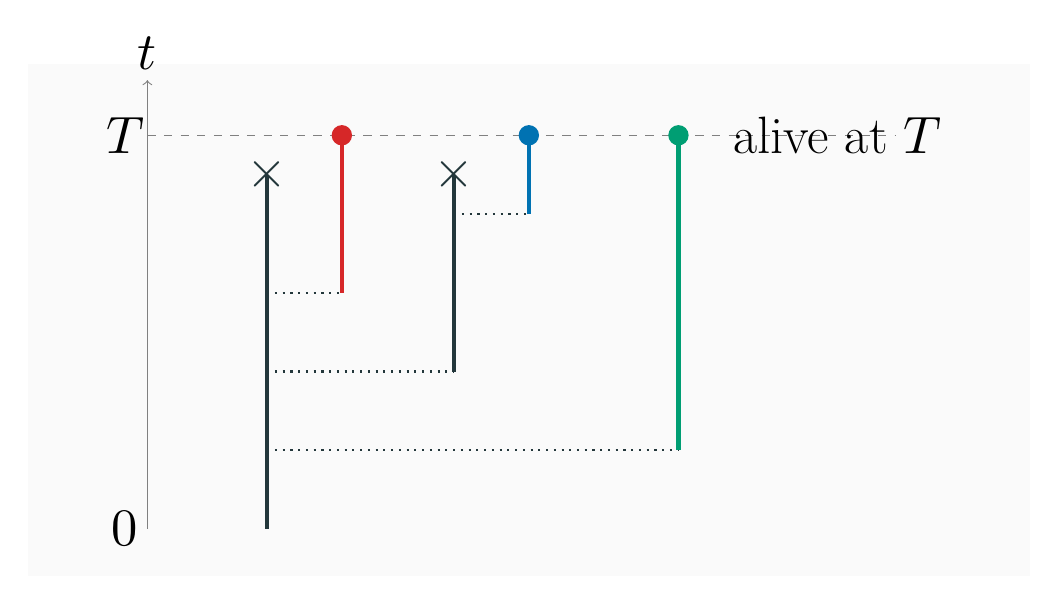
\begin{tikzpicture}[xscale=1.9, yscale=1.0, font=\fontsize{19pt}{23pt}\selectfont]
  \fill[paper] (-0.6,-0.6) rectangle (6.1,5.9);

  % Time axis and the observation time T
  \draw[->, gray] (0.2,0) -- (0.2,5.7) node[above, black] {$t$};
  \node[left] at (0.2,0) {$0$};
  \node[left] at (0.2,5) {$T$};
  \draw[dashed, gray] (0.2,5) -- (5.2,5);

  % Births (dotted) and lifelines
  \draw[thick, dotted, ink]
    (1,1) -- (3.75,1)
    (1,2) -- (2.25,2)
    (1,3) -- (1.5,3)
    (2.25,4) -- (2.75,4);
  \draw[very thick, ink] (1,0) -- (1,4.5) (2.25,2) -- (2.25,4.5);
  \node[ink] at (1,4.5) {$\times$};
  \node[ink] at (2.25,4.5) {$\times$};
  \draw[ultra thick, \sa] (2.75,4) -- (2.75,5);
  \draw[ultra thick, \sb] (1.5,3) -- (1.5,5);
  \draw[ultra thick, \sc] (3.75,1) -- (3.75,5);

  % Individuals alive at T
  \node[circle, fill=\sa, opacity=\dotop, inner sep=2.6pt] at (2.75,5) {};
  \node[circle, fill=\sb, opacity=\dotop, inner sep=2.6pt] at (1.5,5) {};
  \node[circle, fill=\sc, opacity=\dotop, inner sep=2.6pt] at (3.75,5) {};
  \node[anchor=west, opacity=\dotop] at (4.05,5.0) {alive at $T$};
\end{tikzpicture}
\end{document}
"   (k = 1..2)
%   1 the tree        2 the three individuals alive at T coloured and labelled
\documentclass[tikz,border=4pt]{standalone}
\usepackage{xcolor}
\usepackage{libertinus-otf}
\usepackage{unicode-math}
\setmathfont{STIX Two Math}
\definecolor{paper}{HTML}{FAFAFA}
\definecolor{ink}{HTML}{23373B}
\definecolor{blu}{HTML}{0072B2}
\definecolor{red}{HTML}{D62728}
\definecolor{grn}{HTML}{009E73}

\ifcase\stage\or
  \def\sa{ink}\def\sb{ink}\def\sc{ink}\def\dotop{0}\or
  \def\sa{blu}\def\sb{red}\def\sc{grn}\def\dotop{1}\fi

\begin{document}
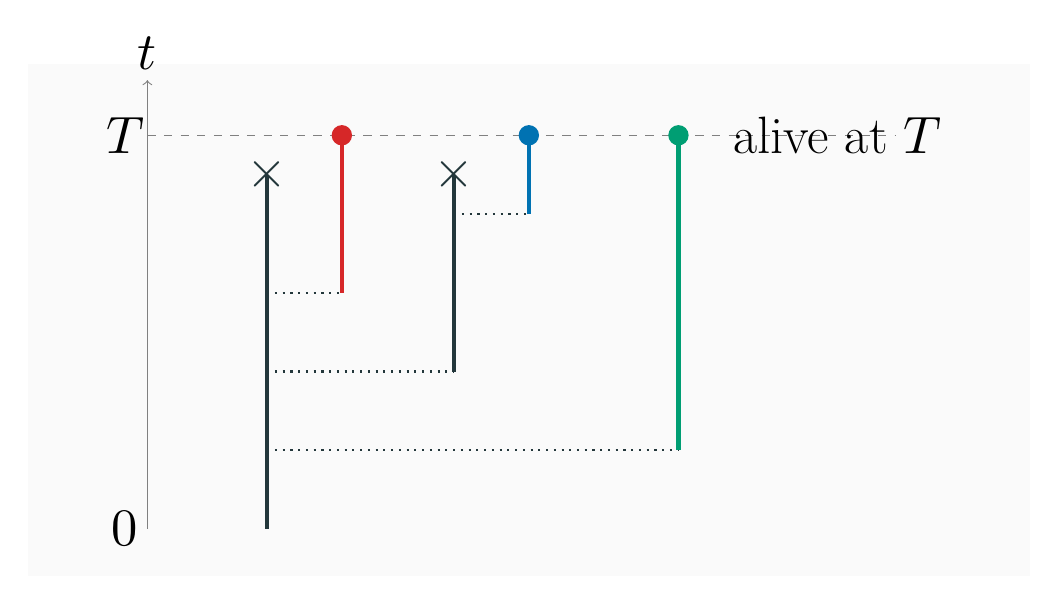
\begin{tikzpicture}[xscale=1.9, yscale=1.0, font=\fontsize{19pt}{23pt}\selectfont]
  \fill[paper] (-0.6,-0.6) rectangle (6.1,5.9);

  % Time axis and the observation time T
  \draw[->, gray] (0.2,0) -- (0.2,5.7) node[above, black] {$t$};
  \node[left] at (0.2,0) {$0$};
  \node[left] at (0.2,5) {$T$};
  \draw[dashed, gray] (0.2,5) -- (5.2,5);

  % Births (dotted) and lifelines
  \draw[thick, dotted, ink]
    (1,1) -- (3.75,1)
    (1,2) -- (2.25,2)
    (1,3) -- (1.5,3)
    (2.25,4) -- (2.75,4);
  \draw[very thick, ink] (1,0) -- (1,4.5) (2.25,2) -- (2.25,4.5);
  \node[ink] at (1,4.5) {$\times$};
  \node[ink] at (2.25,4.5) {$\times$};
  \draw[ultra thick, \sa] (2.75,4) -- (2.75,5);
  \draw[ultra thick, \sb] (1.5,3) -- (1.5,5);
  \draw[ultra thick, \sc] (3.75,1) -- (3.75,5);

  % Individuals alive at T
  \node[circle, fill=\sa, opacity=\dotop, inner sep=2.6pt] at (2.75,5) {};
  \node[circle, fill=\sb, opacity=\dotop, inner sep=2.6pt] at (1.5,5) {};
  \node[circle, fill=\sc, opacity=\dotop, inner sep=2.6pt] at (3.75,5) {};
  \node[anchor=west, opacity=\dotop] at (4.05,5.0) {alive at $T$};
\end{tikzpicture}
\end{document}
"   (k = 1..2)
%   1 the tree        2 the three individuals alive at T coloured and labelled
\documentclass[tikz,border=4pt]{standalone}
\usepackage{xcolor}
\usepackage{libertinus-otf}
\usepackage{unicode-math}
\setmathfont{STIX Two Math}
\definecolor{paper}{HTML}{FAFAFA}
\definecolor{ink}{HTML}{23373B}
\definecolor{blu}{HTML}{0072B2}
\definecolor{red}{HTML}{D62728}
\definecolor{grn}{HTML}{009E73}

\ifcase\stage\or
  \def\sa{ink}\def\sb{ink}\def\sc{ink}\def\dotop{0}\or
  \def\sa{blu}\def\sb{red}\def\sc{grn}\def\dotop{1}\fi

\begin{document}
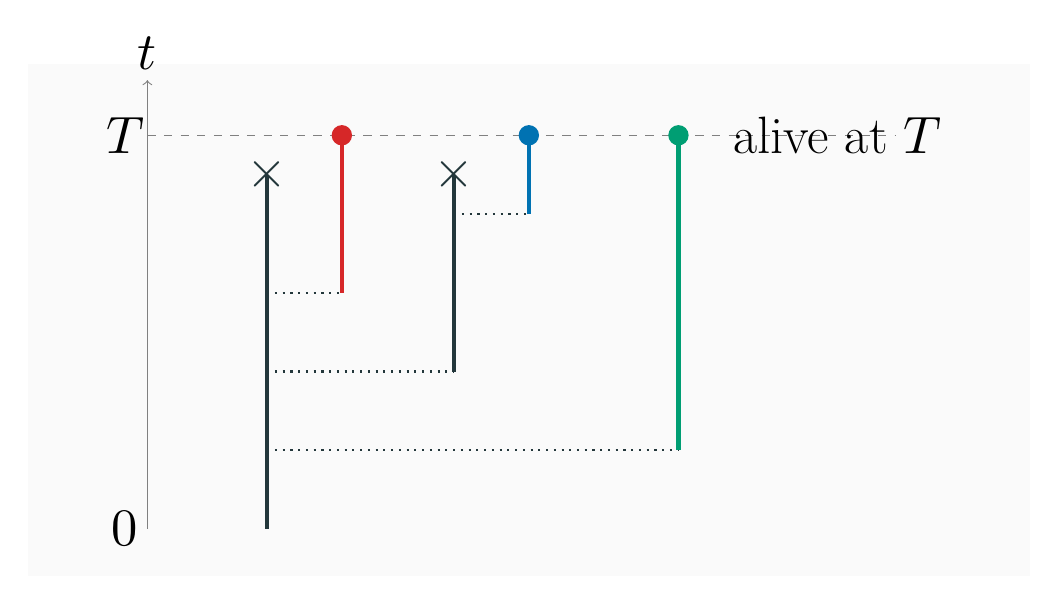
\begin{tikzpicture}[xscale=1.9, yscale=1.0, font=\fontsize{19pt}{23pt}\selectfont]
  \fill[paper] (-0.6,-0.6) rectangle (6.1,5.9);

  % Time axis and the observation time T
  \draw[->, gray] (0.2,0) -- (0.2,5.7) node[above, black] {$t$};
  \node[left] at (0.2,0) {$0$};
  \node[left] at (0.2,5) {$T$};
  \draw[dashed, gray] (0.2,5) -- (5.2,5);

  % Births (dotted) and lifelines
  \draw[thick, dotted, ink]
    (1,1) -- (3.75,1)
    (1,2) -- (2.25,2)
    (1,3) -- (1.5,3)
    (2.25,4) -- (2.75,4);
  \draw[very thick, ink] (1,0) -- (1,4.5) (2.25,2) -- (2.25,4.5);
  \node[ink] at (1,4.5) {$\times$};
  \node[ink] at (2.25,4.5) {$\times$};
  \draw[ultra thick, \sa] (2.75,4) -- (2.75,5);
  \draw[ultra thick, \sb] (1.5,3) -- (1.5,5);
  \draw[ultra thick, \sc] (3.75,1) -- (3.75,5);

  % Individuals alive at T
  \node[circle, fill=\sa, opacity=\dotop, inner sep=2.6pt] at (2.75,5) {};
  \node[circle, fill=\sb, opacity=\dotop, inner sep=2.6pt] at (1.5,5) {};
  \node[circle, fill=\sc, opacity=\dotop, inner sep=2.6pt] at (3.75,5) {};
  \node[anchor=west, opacity=\dotop] at (4.05,5.0) {alive at $T$};
\end{tikzpicture}
\end{document}
"   (k = 1..2)
%   1 the tree        2 the three individuals alive at T coloured and labelled
\documentclass[tikz,border=4pt]{standalone}
\usepackage{xcolor}
\usepackage{libertinus-otf}
\usepackage{unicode-math}
\setmathfont{STIX Two Math}
\definecolor{paper}{HTML}{FAFAFA}
\definecolor{ink}{HTML}{23373B}
\definecolor{blu}{HTML}{0072B2}
\definecolor{red}{HTML}{D62728}
\definecolor{grn}{HTML}{009E73}

\ifcase\stage\or
  \def\sa{ink}\def\sb{ink}\def\sc{ink}\def\dotop{0}\or
  \def\sa{blu}\def\sb{red}\def\sc{grn}\def\dotop{1}\fi

\begin{document}
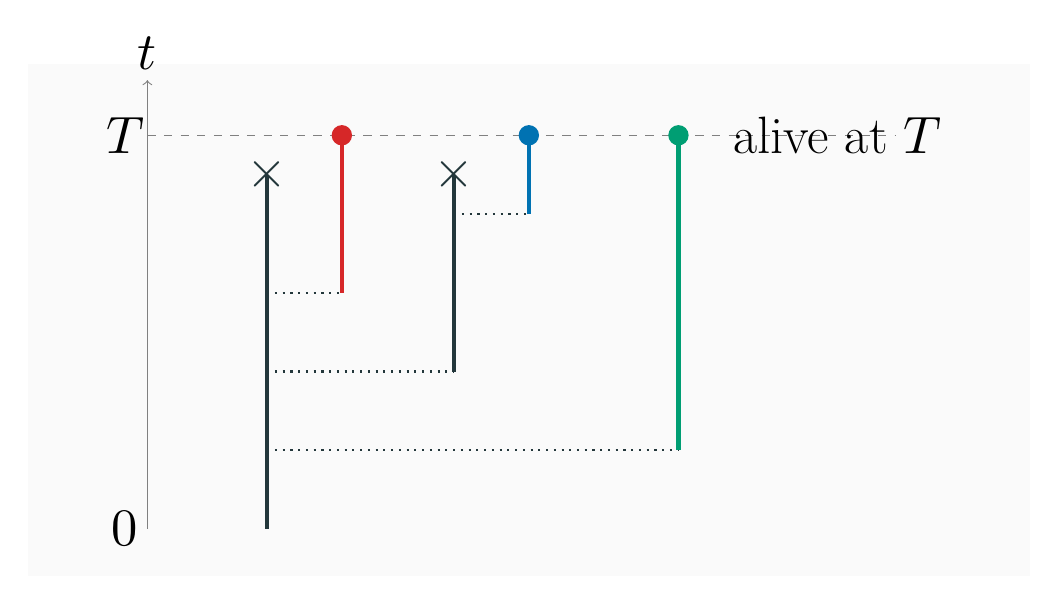
\begin{tikzpicture}[xscale=1.9, yscale=1.0, font=\fontsize{19pt}{23pt}\selectfont]
  \fill[paper] (-0.6,-0.6) rectangle (6.1,5.9);

  % Time axis and the observation time T
  \draw[->, gray] (0.2,0) -- (0.2,5.7) node[above, black] {$t$};
  \node[left] at (0.2,0) {$0$};
  \node[left] at (0.2,5) {$T$};
  \draw[dashed, gray] (0.2,5) -- (5.2,5);

  % Births (dotted) and lifelines
  \draw[thick, dotted, ink]
    (1,1) -- (3.75,1)
    (1,2) -- (2.25,2)
    (1,3) -- (1.5,3)
    (2.25,4) -- (2.75,4);
  \draw[very thick, ink] (1,0) -- (1,4.5) (2.25,2) -- (2.25,4.5);
  \node[ink] at (1,4.5) {$\times$};
  \node[ink] at (2.25,4.5) {$\times$};
  \draw[ultra thick, \sa] (2.75,4) -- (2.75,5);
  \draw[ultra thick, \sb] (1.5,3) -- (1.5,5);
  \draw[ultra thick, \sc] (3.75,1) -- (3.75,5);

  % Individuals alive at T
  \node[circle, fill=\sa, opacity=\dotop, inner sep=2.6pt] at (2.75,5) {};
  \node[circle, fill=\sb, opacity=\dotop, inner sep=2.6pt] at (1.5,5) {};
  \node[circle, fill=\sc, opacity=\dotop, inner sep=2.6pt] at (3.75,5) {};
  \node[anchor=west, opacity=\dotop] at (4.05,5.0) {alive at $T$};
\end{tikzpicture}
\end{document}
